\documentclass{article}

% if you need to pass options to natbib, use, e.g.:
%     \PassOptionsToPackage{numbers, compress}{natbib}
% before loading neurips_2024


% ready for submission
% \usepackage{neurips_2024}


% to compile a preprint version, e.g., for submission to arXiv, add add the
% [preprint] option:
    % \usepackage[preprint]{neurips_2024}


% to compile a camera-ready version, add the [final] option, e.g.:
    \usepackage[final]{neurips_2024}


% to avoid loading the natbib package, add option nonatbib:
   % \usepackage[nonatbib]{neurips_2024}


\usepackage[utf8]{inputenc} % allow utf-8 input
\usepackage[T1]{fontenc}    % use 8-bit T1 fonts
\PassOptionsToPackage{hyphens}{url}\usepackage{hyperref}  % hyperlinks
\usepackage{url}            % simple URL typesetting
\usepackage{booktabs}       % professional-quality tables
\usepackage{amsfonts}       % blackboard math symbols
\usepackage{nicefrac}       % compact symbols for 1/2, etc.
\usepackage{microtype}      % microtypography
\usepackage{xcolor}         % colors
\usepackage[hang,flushmargin]{footmisc}
\usepackage{lipsum}
\usepackage{wrapfig}



\title{Trajectory Analysis in Cell Development}


% The \author macro works with any number of authors. There are two commands
% used to separate the names and addresses of multiple authors: \And and \AND.
%
% Using \And between authors leaves it to LaTeX to determine where to break the
% lines. Using \AND forces a line break at that point. So, if LaTeX puts 3 of 4
% authors names on the first line, and the last on the second line, try using
% \AND instead of \And before the third author name.


\author{%
  Andrew D. Bevington \\
  % Department of Computer Science\\
  Boston College\\
  Chestnut Hill, MA 02467\\
  \texttt{bevingta@bc.edu} \\
  % examples of more authors
  \And
  Charles Y. Kastrud \\
  % Department of Computer Science\\
  Boston College\\
  Chestnut Hill, MA 02467\\
  \texttt{kastrud@bc.edu} \\
  \And
  Andrew Q. Pham \\
  % Department of Computer Science\\
  Boston College\\
  Chestnut Hill, MA 02467\\
  \texttt{phamao@bc.edu} \\
  \And
  Markus D. Sujansky \\
  % Department of Computer Science\\
  Boston College\\
  Chestnut Hill, MA 02467\\
  \texttt{sujansky@bc.edu} \\
  % \And
  % Coauthor \\
  % Affiliation \\
  % Address \\
  % \texttt{email} \\
}

\usepackage{amsmath,stmaryrd,graphicx}

\makeatletter
\newcommand{\fixed@sra}{$\vrule height 2\fontdimen22\textfont2 width 0pt\shortrightarrow$}
\newcommand{\shortarrow}[1]{%
  \mathrel{\text{\rotatebox[origin=c]{\numexpr#1*45}{\fixed@sra}}}%
}
\makeatother

\begin{document}


\maketitle


\begin{abstract}
  In the field of molecular biology, single-cell RNA sequencing (scRNA-seq) has allowed for the profiling of gene expression at the cellular level; however, limitations such as long turnaround times on sample sequences hinder real-life application. This project seeks to explore how trajectory analysis can be used to construct a timeline-independent analysis of a cell's developmental pathway, specifically for use in white and red blood cell development. Using publicly available data from the Paul15 dataset available through Scanpy, trajectory analysis is applied to investigate blood cell development, and their progression within the human body. Tools such as Scanpy and API-based data acquisition address obstacles in data processing, normalization, and integration; this project also investigates biases that can be found in trajectory models like representation and measurement bias. We aim to asses how well trajectory analysis can be used as a tool for understanding cell development and its applications in precision medicine and treatment whilst maintaining ethical concerns around privacy and equity in healthcare models as a top priority.
  
  % The abstract paragraph should be indented \nicefrac{1}{2}~inch (3~picas) on both the left- and right-hand margins. Use 10~point type, with a vertical spacing (leading) of 11~points.  The word \textbf{Abstract} must be centered, bold, and in point size 12. Two line spaces precede the abstract. The abstract must be limited to one paragraph.
\end{abstract}


\section{Background}
RNA sequencing is a technique wherein the number of sequences per gene per cell in a sample is isolated in order to better understand and hopefully modify cell behavior. Haque, et al. goes over how scRNA-seq allows for the comparison of transcriptomes between individual cells, transcriptomes being the RNA sequences that are created from a portion of a genome, the complete set of DNA in an organism contained within every cell in said organism. The investigation of these differences lends itself to the identification of otherwise undetectable cell populations that could potentially be harmful, such as malignant tumors.

\begin{figure}[h]
\centering
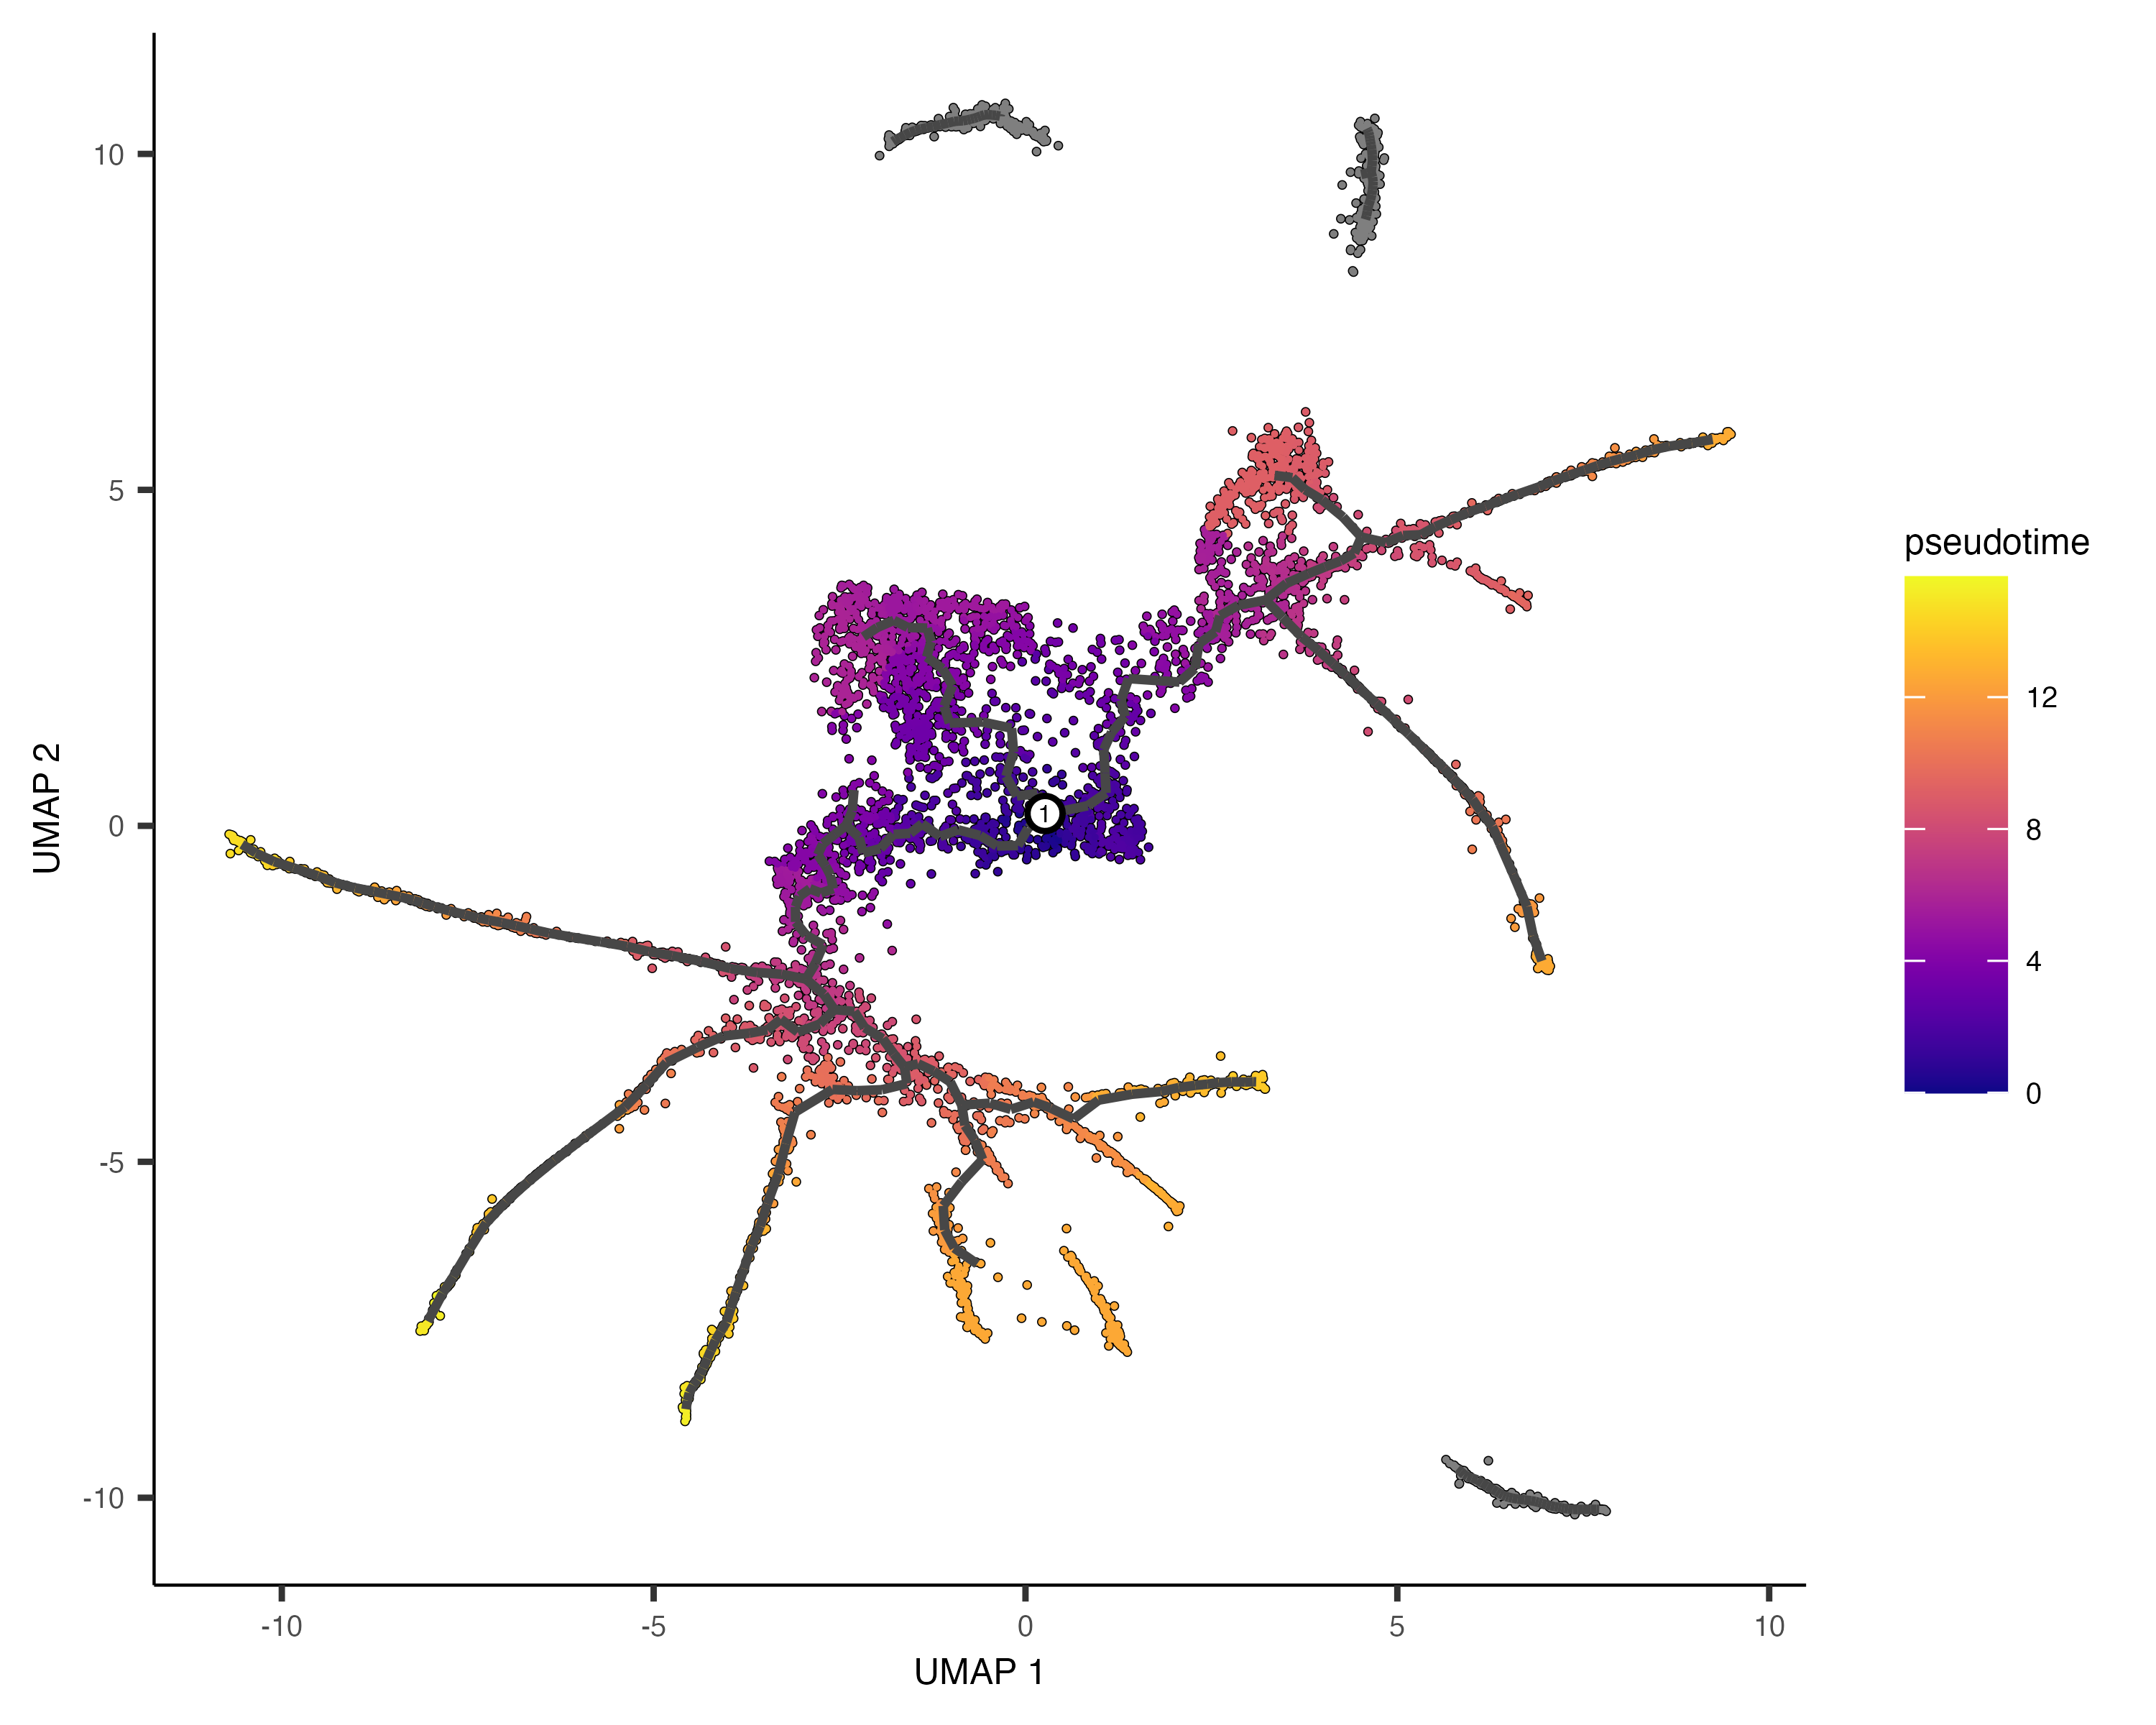
\includegraphics[width=0.5\textwidth]{./images/umap.png}
\caption{Visual representation of an Example Trajectory Plot. Each point in the plot represents a cell / principal component of cells.}
\end{figure}

scRNA-seq functions by taking a "snapshot" of what genes are active or inactive. When a cell expresses genes, it transcribes a copy of the genome into mRNA; variability among cells comes because not all genes are active in a cell at any given time. Their expression is selective and context-dependent, meaning typically only genes that are relevant to a cell's function or a response to outside stimuli/stress are transcribed. Factors like a cell's environment, signaling molecules, or developmental stage can either activate or repress specific genes. As an example, Gregg L. Semenza found that in cancer cells, hypoxia can activate the genes that promote the formation of new blood vessels, angiogenesis, and deactivate genes controlling cell cycle arrest. scRNA-seq isolates individual cells from a sample, capturing their RNA content in a specific moment in time. This RNA is then sequenced, identified, and quantified. RNA abundance reflects gene activity; higher levels of RNA therefore indicate a stronger gene expression.

Within the realm of cancer treatment, scRNA-seq assists in identifying trends in how tumorous cells respond to treatments at the molecular level. Studies such as Patel, et al. and Kinker, et al. reveal how scRNA-seq is used to identify immune and stromal cell interactions that can inform therapy resistance across multiple types of cancers. Since tumors are made up of a variety of different cell populations with unique gene expression profiles, scRNA-seq is capable of identifying subpopulations of problematic cancer cells, such as those with increased drug resistance or more aggressive growth tendencies. It also enables the progression mapping of tumors, allowing researchers to see how they react to treatments; by following the changes in gene expression following chemotherapy for example, one would be able to identify the pathways that develop drug resistance. By profiling and identifying the "traits" of a cell of interest, opportunities for more specialized treatment are growing; biomarkers that indicate the level of patient response to a given treatment, evaluation of immune cell reaction to a treatment, combination therapies, and personally specialized treatment approaches are all made possible through scRNA-seq.

% By producing gene expression profiles, researchers are able to determine whether individual genes are "on" or "off" in a given sample, as genes are "expressed" upon being transcribed into RNA.

It should be noted that, depending on the scRNA-seq protocol used, the level of detail acquired from mRNA data can vary, as discussed by Ziegenhain, et al. and Svensson, et al. This includes features such as how many genes and how many of their transcripts can be detected, whether a specific gene of interest is expressed, whether differential splicing has occurred, etc.

One workaround to this issue is via a method known as trajectory analysis. Trajectory analysis is a widely applicable computational technique that analyzes the course of a measured variable over age or time. Traditional methods such as hierarchical modeling and latent curve analysis similarly measure the relationship between the trajectory of variables and how co-variates may affect them; however, trajectory analysis differs from them by assuming the population is composed of multiple distinct groups, each having a different underlying trajectory instead of using co-variates as an explanation for variability in the estimated population average trajectory. The idea behind trajectory analysis is that it captures all naive, intermediate, and mature cell states; i.e., within a single sample, there is a continuum of cells containing different gene expression profiles which can be used to construct a pseudo-developmental trajectory.

We can visualize this with the shape of a trident; given that 10,000 cells from 5 different samples make up the physical form of the trident, we can identify how similar any particular cell's gene expression is with another. The cells at the lowest point of the trident's handle are the ones least affected by whatever outside influence is being placed on them; the cells directly above these cells are considered to be most similar in terms of gene expression. This trend continues upwards along the handle, where each set of cells is most similar to its immediate upper and lower neighbors, using an unsupervised K-Nearest Neighbors approach. The neck and three separate prongs of the trident represent where whatever outside influence imposed on the cells caused them to split into three differing identities. The tips of each prong represent the most developed cells in relation to their least-affected counterparts at the bottom of the handle.

By combining scRNA-seq and trajectory analysis, we are capable of creating timeline-independent analyses of cell changes across treatments, injuries, and any other relevant contexts in which cell expression profile could potentially be altered.

\section{Motivation}
Trajectory analysis, although seeing a steady increase in utilization within the fields of cancer research and treatment, remains outside mainstream clinical usage. When cell expression is altered due to treatment, injury, or any other relevant context, trajectory analysis allows us to create a timeline-independent analysis in order to track development of said cell. By seeing how cells respond to a specific stimuli, trajectory analysis can be applied for treatment level assistance, like cancer tracking, treatment response prediction, and identifiers of drug resistance. However, it should be kept in mind that this method of modeling is prone to bias like any other. One main focus of this project is to analyze bias in labeling when there are over and under-represented types of cells. It is common that when there are some types which are highly prevalent in test data sets, these types are seen as more common and overrepresented in the training data. There is also a possibility for representation and measurement bias. From the understanding gained through analysis of all three of these forms of bias, future tweaks can be made to either the model or data to make it more fair in a generalized situation.

We see it as important that we explore and understand the implications in overrepresenting and underrepresenting data in this field. By understanding the biases that can be found in trajectory models, we can better understand the limitations of the model and how to address them. We can also aim to further understand how the representation of data manifest itself in the final modeling and if this has an influence on what does and does not get researched. It is important that data is not lost and we want to ensure that all data is represented fairly and accurately in the final model regardless of its prevalence in the training data.

\section{Previous work}
Trajectory analysis continues to grow in its usage in the biomedical field, seeing particular use in cancer research and its applications. Liu, et al. used trajectory analysis to reconstruct the transcriptional development trajectory of malignant epithelial cell; through this, they were able to identify a tumorigenic subcluster regulated by the transcription factor TDFP1, which appears critical for driving tumor progression. They also observed that there was increased infiltration of POSTN+ fibroblasts and SPP1+ macrophages as the tumor advanced in development. These interactions encourage a desmoplastic microenvironment, which reprograms malignant cells in order to enhance tumor progression. During lymph node metastasis, exhausted CXCL13-expressing CD8+ T cells were found to strongly interact with tumor cells, contributing to more aggressive tumor phenotypes, like extranodal expansion. They also identified distinct features of malignant epithelial cells in primary tumors vs. recurrent tumors. Overall, their findings suggested potential targets for therapy at different tumor stages, focusing on precise treatments tailored to the tumor’s microenvironment and cellular states. 

Trapnell, et al. applies a trajectory analysis algorithm known as Monocle to study myoblast differentiation, providing insight on how trajectory analysis can be used to understand the cellular differentiation process. Monocle, as an unsupervised algorithm, orders cells based on their differentiation progress, known as pseudo-time; trajectories are constructed through a high-dimensional space that represents the gene expression profiles of individual cells, allowing for the identification of genes that are activated or repressed at certain stages of differentiation. The algorithm was able to identify eight transcription factors, MZF1, ZIC1, XBP1, USF1, CUX1, ARID5B, POU2F1, and AHR, that had not been previously known to play a role in muscle development. Observation of distinct, sequential waves of transcriptional reconfiguration during myoblast differentiation also suggests an extremely coordinated program of gene regulation during the differentiation process. Analysis of cis-regulatory elements associated with genes in different pseudo-time clusters also revealed more into the regulatory mechanisms behind differentiation, such as how genes that are unregulated during differentiation are enriched for binding motifs of known myogenic regulators like MYOD, MYOG, MEF2, etc.

\section{Modeling}
The term “hematopoiesis” refers to the dynamic cellular process in which self-perpetuation stem cells (HSCs) become more specialized (differentiate) to become various red and white blood cell types. Currently, this process is tracked via a mechanism not accounting for intracellular regulatory mechanisms, which applies discrete thresholds for cell type identification. However, recent evidence relating cell function, differentiation fates, and unexplained heterogeneity within hematopoietic contexts highlights a need for a more appropriate method to track red and white blood cell development in biological contexts (Paul, et al, 2015). Alongside Paul, et al’s alternate methodology, we propose that trajectory analysis is also able to accurately and efficiently track HSC specialization in vivo (within a living organism), making sense of independent non-mixed differentiation pathways and cell types. 

Given the surplus of publicly available trajectory analysis algorithms, we decided not to attempt to create our own, and instead selected ScanPy, a package created in 2018 for a variety of single-cell gene expression analysis including but not limited to trajectory analysis (Wolf, et al, 2018). The workflow used followed the rough shape of Data Preprocessing, Dimensionality Reduction, and finally Trajectory Analysis. Preprocessing allows for removal of cells from the dataset prior to analysis which do not contain enough counts for consideration, or which may contain erroneously high levels of mitochondrial DNA, a marker of a failed single-cell extraction process. Dimensionality Reduction, on the other hand, is purely used to minimize computational strain, as most scRNA-seq datasets contain thousands of cells, each with their own expression data. In the case of ScanPy, Principal Component Analysis (PCA) is used to identify the main axes of variances and effectively de-noise the data. Finally, the trajectory analysis step runs the algorithm and visualizes the results. 

\subsection{Shortcomings}
Analyzing the data representation revealed significant disparities in the information contained in the dataset. For these measurements, a ratio of 1.00 would indicate perfect parity between expected and observed frequencies. However, deviations were observed across multiple cell populations. Overrepresented groups with a ratio > 1.5 included monocytes (14Mo, ratio = 2.596), erythrocytes (2Ery), basophils (13Baso), and erythrocytes (3Ery). On the other side, underrepresented groups with a ratio < 0.5 constined eosinophils (18Eos, ratio = 0.063), neutrophils (17Neu), dendritic cells (11DC), and lymphocytes (19Lymph).

The disparity ratio $\delta$ defined as:
$[\delta = \frac{\text{max}(\text{representation ratio})}{\text{min}(\text{representation ratio})} = \frac{2.596}{0.063} \approx 41.21]$
indicates a severe representation imbalance within the dataset. While this is concerning from a data perspective, it is representative of the general cell population. The issue is that this disparity, while present in the natural world, is harmful to a model learning to predict information.

These disparities can cause issues which we will see cascade through the medical world if used as the only source of truth in prediction. When certain cell types, such as 14Mo, are overrepresented, the models become disproportionately prepared to predict these populations. This could lead to more common cell types being better predicted while negatively impacting the more rare cell types. This is most often seen in the initial analysis stages where underrepresented cell types output less predictive information on their characteristics and impact.

The implication of these biases extends beyond data analysis and makes its way into the world of medical research. From what we have seen, research proposals have tended to gravitate towards more well-represented cell types. The availability of data, enhanced statistical power in experimental designs, higher probability of successful publication, and increased likelihood of significant results all contribute to this trend. For instance, research on eosinophil-mediated allergic responses may receive less attention despite the clinical significance just because of the underrepresentation in datasets and therefore the underrepresentation of information on the cells as a whole. This creates a cycle where research becomes increasingly skewed toward already well-studied cell populations.

This bias particularly impacts machine learning applications in medical research, where models trained on imbalanced datasets may overfit for common cell types and show reduced sensitivity to rare cell types leading to systematic blind spots in edge case detection and biased weightings of feature importance. These effects can significantly impact the model's ability to generalize across diverse cell populations and rare cell states.


\section{Results}
In the context of medical discovery, this presents a significant challenge. While predictive models optimize for frequently observed patterns, medical research often requires particular attention to outliers and minimally represented systems. Because of this, normal machine learning models may be fundamentally misaligned with what the medical field needs and alternative methods must be explored in order to allow for the complexity and edge detection needed.

We found that there are a few avenues of exploration for alleviating these concerns. We theorized that stratifying data collection and processing would help the more underrepresented cell types to get the attention they need. Weighted loss functions can also be used to give rare cell types more of a presence in the training steps. Synthetic data generation techniques may be used to create more of a population for the smaller cell types while maintaining their general characteristics. However, it is important to continue testing to ensure that rare cell types get the weight necessary to be considered, but not too much weight that they themselves become overrepresented in relation to their real population size. 


\begin{figure}[h]
\centering
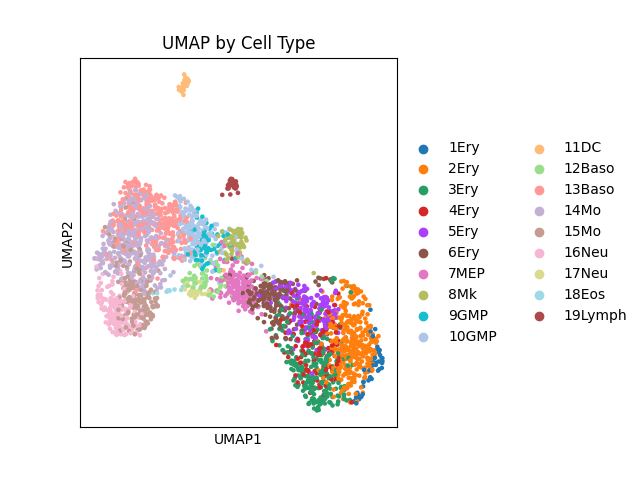
\includegraphics[width=0.5\textwidth]{./images/umap_cell_types.png}
\caption{Visual representation of an Example Trajectory Plot. Each point in the plot represents a cell / principal component of cells.}
\end{figure}


Even before running trajectory analysis, the output from the dimensionality reduction step already suggested that there was more than met the eye within the dataset. Figure 2 shows a UMAP, which plots the first two Principal Components against one another. The details are somewhat complicated, but all that needs to be known to understand the graph is as follows: 1) Each dot on the graph represents a cell or group of cells, and 2) The closer two points are to one another on the graph, the more similar they are in gene expression. The naive approach to understanding described as a cause for change in Paul, et al, assumes equal “distance” between HSC and terminally differentiated cell types. That is, each cell type which can come to be from an HSC differentiating is equally “different” from that HSC. However, a quick glance at the UMAP shows that two types, 11DC (Dendritic Cells) and 19Lymph (Lymphoid Cells) are clearly separate from the pack. 


\begin{figure}[h]
\centering
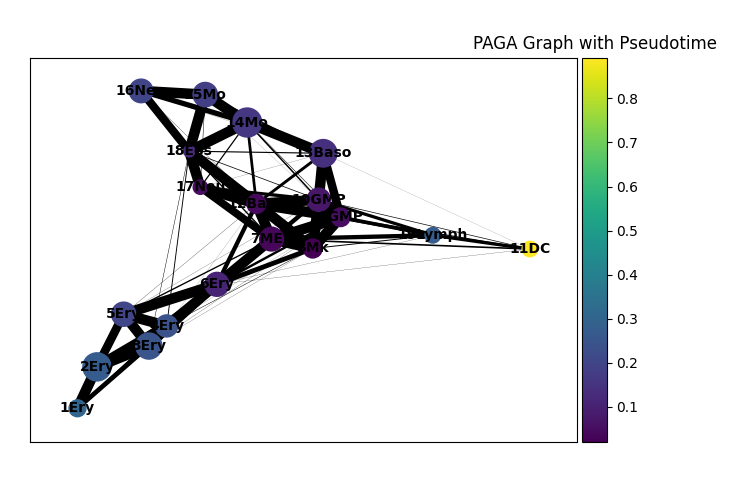
\includegraphics[width=0.5\textwidth]{./images/paga_graph_pseudotime.png}
\caption{Visual representation of an Example Trajectory Plot. Each point in the plot represents a cell / principal component of cells.}
\end{figure}


This analysis is further underscored by the trajectory plot shown in Figure 3. There are three clear trajectories originating from a central mass at Pseudotime 0. The first lineage ($\shortarrow{3}$) terminates as a Neutrophil (Neu), the second ($\shortarrow{5}$) as an Erythrocyte (Ery), and the third ($\shortarrow{0}$) as a Dendritic Cell (DC). Of these, the lineage of most interest is that of the Dendritic Cells, as the pseudotime variable at terminal identity (~0.9-1.0) suggests a much more involved differentiation process in comparison to those of the first two lineages (~0.25 and ~0.35 respectively). While definite reasons for this difference cannot be drawn from the graph alone, one might hypothesize that the DC differentiation pathway relies on distinct developmental requirements, which may be more reliant on either environmental or intracellular conditions than the other cell types. Further, more directed research would need to be done to confirm or refute such a claim.

In any case, it is clear that trajectory analysis is capable of increased sensitivity in detecting cellular changes throughout a biological process (like differentiation) when compared to more traditional gene-recognition methods, as described in Paul, et al. Heavily reliant on the data itself, however, it is still vulnerable to biases and fairness issues relating to access and privacy.


\section{Conclusion}
Trajectory analysis is immensely beneficial in identifying complex biological processes, able to track the transformation of cell types over time.  The results of our study confirm this effectiveness.  Dendritic cells, for example, followed a more intricate process of differentiation than neutrophils and erythrocytes.  This highlights how accurate trajectory analysis is in tracking detailed cellular changes.  While this technology has transformative potential, the underlying issue of dataset bias is of great concern.  Our study revealed significant disparity ratios, with some as high as 41.21.  In order for trajectory analysis to produce fair and unbiased results, datasets must be balanced and representative of all cell types.

In the context of medical discovery, this presents a significant challenge. While predictive models optimize for frequently observed patterns, medical research often requires particular attention to outliers and minimally represented systems. Because of this, normal machine learning models may be fundamentally misaligned with what the medical field needs and alternative methods must be explored in order to allow for the complexity and edge detection needed.

We found that there are a few avenues of exploration for alleviating these concerns. We theorized that stratifying data collection and processing would help the more underrepresented cell types to get the attention they need. Weighted loss functions can also be used to give rare cell types more of a presence in the training steps. Synthetic data generation techniques may be used to create more of a population for the smaller cell types while maintaining their general characteristics. However, it is important to continue testing to ensure that rare cell types get the weight necessary to be considered, but not too much weight that they themselves become overrepresented in relation to their real population size. 


\subsection{Takeaways}
Trajectory analysis is undoubtedly a beneficial tool in a healthcare setting.  However, this technology, as well as tech-enabled healthcare as a whole, raises some serious legal and ethical concerns in its application.  As machine learning techniques continue to shape the world of healthcare, data privacy and security must be of the utmost concern.

Any machine learning application cannot run without data.  In order to learn and make accurate predictions, there needs to be a large dataset for the model to be trained on.  In the setting of healthcare, however, the privacy and security of this data must be ensured.  Dealing with personal, sensitive information like health data requires strong anonymization protocols to protect the identities of those supplying the data, as nobody wants their own personal data to be exposed to the public.  The United States, as well as the EU, have regulatory safeguards in place to protect individuals’ medical data.  In the US, HIPAA is the governing legislation.  In regards to the collection and use of personal medical information, HIPAA requires data to be properly anonymized before being used.  This involved removing specific identifiers that can be used to track the identity of the person supplying the data.  Specific identifiers include, but are not limited to: names, social security numbers, birth dates, past medical records, etc (GenInvo).  The EU follows the GDPR to protect the confidentiality of patient data.  While they are both aimed at the same goal, The GDPR offers more data protections than HIPAA.  GDPR also requires the stripping of specific identifiers, but it also has more strict requirements for explicit consent of data use.  Under GDPR, all data collected must be done so at the expressed consent of the patient, whereas HIPAA includes some exceptions that allow the use of medical data without explicit consent from the patient (Dougherty).

\subsection{Recommendations}
While data anonymization is a widely used method to protect individual medical information, there is emerging technology today that threatens the security of this method.  sciences.   There are algorithms that exist today that are able to re-identify the identity of an individual based on anonymized medical data. Researchers conducting a 2018 study found that “an algorithm could be used to re-identify 85.6\% of adults and 69.8\% of children in a physical activity cohort study, despite the supposed removal of identifiers of protected health information” (Murdoch).  This danger of re-identification is a massive legal and ethical issue, especially in the context of trajectory analysis, which relies upon datasets containing personal medical information to operate.  As the capabilities of machine learning continue to evolve, the legislation protecting data must keep up to ensure that individuals’ rights to privacy are adequately protected.  Any technology that is used to make decisions that impact the health and care of patients must be tightly regulated.  And as technological advancements tend to outpace corresponding legislation, there must be a push to ensure that tech-enabled healthcare is subject to strict regulation from the government.
\newpage

[1] Alexander, J.A.\ \& Mozer, M.C.\ (1995) Template-based algorithms for
connectionist rule extraction. In G.\ Tesauro, D.S.\ Touretzky and T.K.\ Leen
(eds.), {\it Advances in Neural Information Processing Systems 7},
pp.\ 609--616. Cambridge, MA: MIT Press.


[2] Bower, J.M.\ \& Beeman, D.\ (1995) {\it The Book of GENESIS: Exploring
  Realistic Neural Models with the GEneral NEural SImulation System.}  New York:
TELOS/Springer--Verlag.


[3] Hasselmo, M.E., Schnell, E.\ \& Barkai, E.\ (1995) Dynamics of learning and
recall at excitatory recurrent synapses and cholinergic modulation in rat
hippocampal region CA3. {\it Journal of Neuroscience} {\bf 15}(7):5249-5262.

[4] Haque, A., Engel, J., Teichmann, S.A. et al. A practical guide to single-cell RNA-sequencing for biomedical research and clinical applications. Genome Med 9, 75 (2017). https://doi.org/10.1186/s13073-017-0467-4

[5] Semenza, G. Targeting HIF-1 for cancer therapy. Nat Rev Cancer 3, 721–732 (2003). https://doi.org/10.1038/nrc1187

[6] Svensson, V., Vento-Tormo, R. \& Teichmann, S. Exponential scaling of single-cell RNA-seq in the past decade. Nat Protoc 13, 599–604 (2018). https://doi.org/10.1038/nprot.2017.149

[7] Patel AP, Tirosh I, Trombetta JJ, Shalek AK, Gillespie SM, Wakimoto H, Cahill DP, Nahed BV, Curry WT, Martuza RL, Louis DN, Rozenblatt-Rosen O, Suvà ML, Regev A, Bernstein BE. Single-cell RNA-seq highlights intratumoral heterogeneity in primary glioblastoma. Science. 2014 Jun 20;344(6190):1396-401. doi: 10.1126/science.1254257. Epub 2014 Jun 12. PMID: 24925914; PMCID: PMC4123637.

[8] Kinker, G.S., Greenwald, A.C., Tal, R. et al. Pan-cancer single-cell RNA-seq identifies recurring programs of cellular heterogeneity. Nat Genet 52, 1208–1218 (2020). https://doi.org/10.1038/s41588-020-00726-6

[9] Christoph Ziegenhain, Beate Vieth, Swati Parekh, Björn Reinius, Amy Guillaumet-Adkins, Martha Smets, Heinrich Leonhardt, Holger Heyn, Ines Hellmann, Wolfgang Enard, Comparative Analysis of Single-Cell RNA Sequencing Methods, Molecular Cell, Volume 65, Issue 4, 2017, Pages 631-643.e4, ISSN 1097-2765, https://doi.org/10.1016/j.molcel.2017.01.023.

[10] Svensson, V., Natarajan, K., Ly, LH. et al. Power analysis of single-cell RNA-sequencing experiments. Nat Methods 14, 381–387 (2017). https://doi.org/10.1038/nmeth.4220

[11] Liu, Z.L., Meng, X.Y., Bao, R.J. et al. Single cell deciphering of progression trajectories of the tumor ecosystem in head and neck cancer. Nat Commun 15, 2595 (2024). https://doi.org/10.1038/s41467-024-46912-6

[12] Trapnell C, Cacchiarelli D, Grimsby J, Pokharel P, Li S, Morse M, Lennon NJ, Livak KJ, Mikkelsen TS, Rinn JL. The dynamics and regulators of cell fate decisions are revealed by pseudotemporal ordering of single cells. Nat Biotechnol. 2014 Apr;32(4):381-386. doi: 10.1038/nbt.2859. Epub 2014 Mar 23. PMID: 24658644; PMCID: PMC4122333.


\end{document}
